\chapter{La Mazzolata}

Gentlemen,” said the Count of Monte Cristo as he entered, “I pray you
excuse me for suffering my visit to be anticipated; but I feared to
disturb you by presenting myself earlier at your apartments; besides,
you sent me word that you would come to me, and I have held myself at
your disposal.”

“Franz and I have to thank you a thousand times, count,” returned
Albert; “you extricated us from a great dilemma, and we were on the
point of inventing a very fantastic vehicle when your friendly
invitation reached us.”

“Indeed,” returned the count, motioning the two young men to sit down.
“It was the fault of that blockhead Pastrini, that I did not sooner
assist you in your distress. He did not mention a syllable of your
embarrassment to me, when he knows that, alone and isolated as I am, I
seek every opportunity of making the acquaintance of my neighbors. As
soon as I learned I could in any way assist you, I most eagerly seized
the opportunity of offering my services.”

The two young men bowed. Franz had, as yet, found nothing to say; he
had come to no determination, and as nothing in the count’s manner
manifested the wish that he should recognize him, he did not know
whether to make any allusion to the past, or wait until he had more
proof; besides, although sure it was he who had been in the box the
previous evening, he could not be equally positive that this was the
man he had seen at the Colosseum. He resolved, therefore, to let things
take their course without making any direct overture to the count.
Moreover, he had this advantage, he was master of the count’s secret,
while the count had no hold on Franz, who had nothing to conceal.
However, he resolved to lead the conversation to a subject which might
possibly clear up his doubts.

“Count,” said he, “you have offered us places in your carriage, and at
your windows in the Rospoli Palace. Can you tell us where we can obtain
a sight of the Piazza del Popolo?”

“Ah,” said the count negligently, looking attentively at Morcerf, “is
there not something like an execution upon the Piazza del Popolo?”

“Yes,” returned Franz, finding that the count was coming to the point
he wished.

“Stay, I think I told my steward yesterday to attend to this; perhaps I
can render you this slight service also.”

He extended his hand, and rang the bell thrice.

“Did you ever occupy yourself,” said he to Franz, “with the employment
of time and the means of simplifying the summoning your servants? I
have. When I ring once, it is for my valet; twice, for my majordomo;
thrice, for my steward,—thus I do not waste a minute or a word. Here he
is.”

A man of about forty-five or fifty entered, exactly resembling the
smuggler who had introduced Franz into the cavern; but he did not
appear to recognize him. It was evident he had his orders.

“Monsieur Bertuccio,” said the count, “you have procured me windows
looking on the Piazza del Popolo, as I ordered you yesterday.”

“Yes, excellency,” returned the steward; “but it was very late.”

“Did I not tell you I wished for one?” replied the count, frowning.

“And your excellency has one, which was let to Prince Lobanieff; but I
was obliged to pay a hundred——”

“That will do—that will do, Monsieur Bertuccio; spare these gentlemen
all such domestic arrangements. You have the window, that is
sufficient. Give orders to the coachman; and be in readiness on the
stairs to conduct us to it.”

The steward bowed, and was about to quit the room.

“Ah!” continued the count, “be good enough to ask Pastrini if he has
received the \textit{tavoletta}, and if he can send us an account of the
execution.”

“There is no need to do that,” said Franz, taking out his tablets; “for
I saw the account, and copied it down.”

“Very well, you can retire, M. Bertuccio; I need you no longer. Let us
know when breakfast is ready. These gentlemen,” added he, turning to
the two friends, “will, I trust, do me the honor to breakfast with me?”

“But, my dear count,” said Albert, “we shall abuse your kindness.”

“Not at all; on the contrary, you will give me great pleasure. You
will, one or other of you, perhaps both, return it to me at Paris. M.
Bertuccio, lay covers for three.”

He then took Franz’s tablets out of his hand. “‘We announce,’ he read,
in the same tone with which he would have read a newspaper, ‘that
today, the 23rd of February, will be executed Andrea Rondolo, guilty of
murder on the person of the respected and venerated Don César Torlini,
canon of the church of St. John Lateran, and Peppino, called Rocca
Priori, convicted of complicity with the detestable bandit Luigi Vampa,
and the men of his band.’

“Hum! ‘The first will be \textit{mazzolato}, the second \textit{decapitato}.’ Yes,”
continued the count, “it was at first arranged in this way; but I think
since yesterday some change has taken place in the order of the
ceremony.”

“Really?” said Franz.

“Yes, I passed the evening at the Cardinal Rospigliosi’s, and there
mention was made of something like a pardon for one of the two men.”

“For Andrea Rondolo?” asked Franz.

“No,” replied the count, carelessly; “for the other (he glanced at the
tablets as if to recall the name), for Peppino, called Rocca Priori.
You are thus deprived of seeing a man guillotined; but the \textit{mazzolata}
still remains, which is a very curious punishment when seen for the
first time, and even the second, while the other, as you must know, is
very simple. The \textit{mandaïa}\footnote[6]{Guillotine.} never fails, never trembles, never strikes
thirty times ineffectually, like the soldier who beheaded the Count of
Chalais, and to whose tender mercy Richelieu had doubtless recommended
the sufferer. Ah,” added the count, in a contemptuous tone, “do not
tell me of European punishments, they are in the infancy, or rather the
old age, of cruelty.”

“Really, count,” replied Franz, “one would think that you had studied
the different tortures of all the nations of the world.”

“There are, at least, few that I have not seen,” said the count coldly.

“And you took pleasure in beholding these dreadful spectacles?”

“My first sentiment was horror, the second indifference, the third
curiosity.”

“Curiosity—that is a terrible word.”

“Why so? In life, our greatest preoccupation is death; is it not then,
curious to study the different ways by which the soul and body can
part; and how, according to their different characters, temperaments,
and even the different customs of their countries, different persons
bear the transition from life to death, from existence to annihilation?
As for myself, I can assure you of one thing,—the more men you see die,
the easier it becomes to die yourself; and in my opinion, death may be
a torture, but it is not an expiation.”

“I do not quite understand you,” replied Franz; “pray explain your
meaning, for you excite my curiosity to the highest pitch.”

“Listen,” said the count, and deep hatred mounted to his face, as the
blood would to the face of any other. “If a man had by unheard-of and
excruciating tortures destroyed your father, your mother, your
betrothed,—a being who, when torn from you, left a desolation, a wound
that never closes, in your breast,—do you think the reparation that
society gives you is sufficient when it interposes the knife of the
guillotine between the base of the occiput and the trapezal muscles of
the murderer, and allows him who has caused us years of moral
sufferings to escape with a few moments of physical pain?”

“Yes, I know,” said Franz, “that human justice is insufficient to
console us; she can give blood in return for blood, that is all; but
you must demand from her only what it is in her power to grant.”

“I will put another case to you,” continued the count; “that where
society, attacked by the death of a person, avenges death by death. But
are there not a thousand tortures by which a man may be made to suffer
without society taking the least cognizance of them, or offering him
even the insufficient means of vengeance, of which we have just spoken?
Are there not crimes for which the impalement of the Turks, the augers
of the Persians, the stake and the brand of the Iroquois Indians, are
inadequate tortures, and which are unpunished by society? Answer me, do
not these crimes exist?”

“Yes,” answered Franz; “and it is to punish them that duelling is
tolerated.”

“Ah, duelling,” cried the count; “a pleasant manner, upon my soul, of
arriving at your end when that end is vengeance! A man has carried off
your mistress, a man has seduced your wife, a man has dishonored your
daughter; he has rendered the whole life of one who had the right to
expect from Heaven that portion of happiness God has promised to
everyone of his creatures, an existence of misery and infamy; and you
think you are avenged because you send a ball through the head, or pass
a sword through the breast, of that man who has planted madness in your
brain, and despair in your heart. And remember, moreover, that it is
often he who comes off victorious from the strife, absolved of all
crime in the eyes of the world. No, no,” continued the count, “had I to
avenge myself, it is not thus I would take revenge.”

“Then you disapprove of duelling? You would not fight a duel?” asked
Albert in his turn, astonished at this strange theory.

“Oh, yes,” replied the count; “understand me, I would fight a duel for
a trifle, for an insult, for a blow; and the more so that, thanks to my
skill in all bodily exercises, and the indifference to danger I have
gradually acquired, I should be almost certain to kill my man. Oh, I
would fight for such a cause; but in return for a slow, profound,
eternal torture, I would give back the same, were it possible; an eye
for an eye, a tooth for a tooth, as the Orientalists say,—our masters
in everything,—those favored creatures who have formed for themselves a
life of dreams and a paradise of realities.”

“But,” said Franz to the count, “with this theory, which renders you at
once judge and executioner of your own cause, it would be difficult to
adopt a course that would forever prevent your falling under the power
of the law. Hatred is blind, rage carries you away; and he who pours
out vengeance runs the risk of tasting a bitter draught.”

“Yes, if he be poor and inexperienced, not if he be rich and skilful;
besides, the worst that could happen to him would be the punishment of
which we have already spoken, and which the philanthropic French
Revolution has substituted for being torn to pieces by horses or broken
on the wheel. What matters this punishment, as long as he is avenged?
On my word, I almost regret that in all probability this miserable
Peppino will not be beheaded, as you might have had an opportunity then
of seeing how short a time the punishment lasts, and whether it is
worth even mentioning; but, really this is a most singular conversation
for the Carnival, gentlemen; how did it arise? Ah, I recollect, you
asked for a place at my window; you shall have it; but let us first sit
down to table, for here comes the servant to inform us that breakfast
is ready.”

As he spoke, a servant opened one of the four doors of the apartment,
saying:

“\textit{Al suo commodo!}”

The two young men arose and entered the breakfast-room.

During the meal, which was excellent, and admirably served, Franz
looked repeatedly at Albert, in order to observe the impressions which
he doubted not had been made on him by the words of their entertainer;
but whether with his usual carelessness he had paid but little
attention to him, whether the explanation of the Count of Monte Cristo
with regard to duelling had satisfied him, or whether the events which
Franz knew of had had their effect on him alone, he remarked that his
companion did not pay the least regard to them, but on the contrary ate
like a man who for the last four or five months had been condemned to
partake of Italian cookery—that is, the worst in the world.

As for the count, he just touched the dishes; he seemed to fulfil the
duties of a host by sitting down with his guests, and awaited their
departure to be served with some strange or more delicate food. This
brought back to Franz, in spite of himself, the recollection of the
terror with which the count had inspired the Countess G——, and her firm
conviction that the man in the opposite box was a vampire.

At the end of the breakfast Franz took out his watch.

“Well,” said the count, “what are you doing?”

“You must excuse us, count,” returned Franz, “but we have still much to
do.”

“What may that be?”

“We have no masks, and it is absolutely necessary to procure them.”

“Do not concern yourself about that; we have, I think, a private room
in the Piazza del Popolo; I will have whatever costumes you choose
brought to us, and you can dress there.”

“After the execution?” cried Franz.

“Before or after, whichever you please.”

“Opposite the scaffold?”

“The scaffold forms part of the \textit{fête}.”

“Count, I have reflected on the matter,” said Franz, “I thank you for
your courtesy, but I shall content myself with accepting a place in
your carriage and at your window at the Rospoli Palace, and I leave you
at liberty to dispose of my place at the Piazza del Popolo.”

“But I warn you, you will lose a very curious sight,” returned the
count.

“You will describe it to me,” replied Franz, “and the recital from your
lips will make as great an impression on me as if I had witnessed it. I
have more than once intended witnessing an execution, but I have never
been able to make up my mind; and you, Albert?”

“I,” replied the viscount,—“I saw Castaing executed, but I think I was
rather intoxicated that day, for I had quitted college the same
morning, and we had passed the previous night at a tavern.”

“Besides, it is no reason because you have not seen an execution at
Paris, that you should not see one anywhere else; when you travel, it
is to see everything. Think what a figure you will make when you are
asked, ‘How do they execute at Rome?’ and you reply, ‘I do not know!’
And, besides, they say that the culprit is an infamous scoundrel, who
killed with a log of wood a worthy canon who had brought him up like
his own son. \textit{Diable!} when a churchman is killed, it should be with a
different weapon than a log, especially when he has behaved like a
father. If you went to Spain, would you not see the bull-fights? Well,
suppose it is a bull-fight you are going to see? Recollect the ancient
Romans of the Circus, and the sports where they killed three hundred
lions and a hundred men. Think of the eighty thousand applauding
spectators, the sage matrons who took their daughters, and the charming
Vestals who made with the thumb of their white hands the fatal sign
that said, ‘Come, despatch the dying.’”

“Shall you go, then, Albert?” asked Franz.

“\textit{Ma foi}, yes; like you, I hesitated, but the count’s eloquence
decides me.”

“Let us go, then,” said Franz, “since you wish it; but on our way to
the Piazza del Popolo, I wish to pass through the Corso. Is this
possible, count?”

“On foot, yes, in a carriage, no.”

“I will go on foot, then.”

“Is it important that you should go that way?”

“Yes, there is something I wish to see.”

“Well, we will go by the Corso. We will send the carriage to wait for
us on the Piazza del Popolo, by the Via del Babuino, for I shall be
glad to pass, myself, through the Corso, to see if some orders I have
given have been executed.”

“Excellency,” said a servant, opening the door, “a man in the dress of
a penitent wishes to speak to you.”

“Ah! yes,” returned the count, “I know who he is, gentlemen; will you
return to the salon? you will find good cigars on the centre table. I
will be with you directly.”

The young men rose and returned into the salon, while the count, again
apologizing, left by another door. Albert, who was a great smoker, and
who had considered it no small sacrifice to be deprived of the cigars
of the Café de Paris, approached the table, and uttered a cry of joy at
perceiving some veritable \textit{puros}.

“Well,” asked Franz, “what think you of the Count of Monte Cristo?”

“What do I think?” said Albert, evidently surprised at such a question
from his companion; “I think he is a delightful fellow, who does the
honors of his table admirably; who has travelled much, read much, is,
like Brutus, of the Stoic school, and moreover,” added he, sending a
volume of smoke up towards the ceiling, “that he has excellent cigars.”

Such was Albert’s opinion of the count, and as Franz well knew that
Albert professed never to form an opinion except upon long reflection,
he made no attempt to change it.

“But,” said he, “did you observe one very singular thing?”

“What?”

“How attentively he looked at you.”

“At me?”

“Yes.”

Albert reflected. “Ah,” replied he, sighing, “that is not very
surprising; I have been more than a year absent from Paris, and my
clothes are of a most antiquated cut; the count takes me for a
provincial. The first opportunity you have, undeceive him, I beg, and
tell him I am nothing of the kind.”

Franz smiled; an instant after the count entered.

“I am now quite at your service, gentlemen,” said he. “The carriage is
going one way to the Piazza del Popolo, and we will go another; and, if
you please, by the Corso. Take some more of these cigars, M. de
Morcerf.”

“With all my heart,” returned Albert; “Italian cigars are horrible.
When you come to Paris, I will return all this.”

“I will not refuse; I intend going there soon, and since you allow me,
I will pay you a visit. Come, we have not any time to lose, it is
half-past twelve—let us set off.”

All three descended; the coachman received his master’s orders, and
drove down the Via del Babuino. While the three gentlemen walked along
the Piazza di Spagna and the Via Frattina, which led directly between
the Fiano and Rospoli palaces, Franz’s attention was directed towards
the windows of that last palace, for he had not forgotten the signal
agreed upon between the man in the mantle and the Transtevere peasant.

“Which are your windows?” asked he of the count, with as much
indifference as he could assume.

“The three last,” returned he, with a negligence evidently unaffected,
for he could not imagine with what intention the question was put.

Franz glanced rapidly towards the three windows. The side windows were
hung with yellow damask, and the centre one with white damask and a red
cross. The man in the mantle had kept his promise to the Transteverin,
and there could now be no doubt that he was the count.

The three windows were still untenanted. Preparations were making on
every side; chairs were placed, scaffolds were raised, and windows were
hung with flags. The masks could not appear; the carriages could not
move about; but the masks were visible behind the windows, the
carriages, and the doors.

Franz, Albert, and the count continued to descend the Corso. As they
approached the Piazza del Popolo, the crowd became more dense, and
above the heads of the multitude two objects were visible: the obelisk,
surmounted by a cross, which marks the centre of the square, and in
front of the obelisk, at the point where the three streets, del
Babuino, del Corso, and di Ripetta, meet, the two uprights of the
scaffold, between which glittered the curved knife of the \textit{mandaïa}.

At the corner of the street they met the count’s steward, who was
awaiting his master. The window, let at an exorbitant price, which the
count had doubtless wished to conceal from his guests, was on the
second floor of the great palace, situated between the Via del Babuino
and the Monte Pincio. It consisted, as we have said, of a small
dressing-room, opening into a bedroom, and, when the door of
communication was shut, the inmates were quite alone. On chairs were
laid elegant masquerade costumes of blue and white satin.

\begin{figure}[ht]
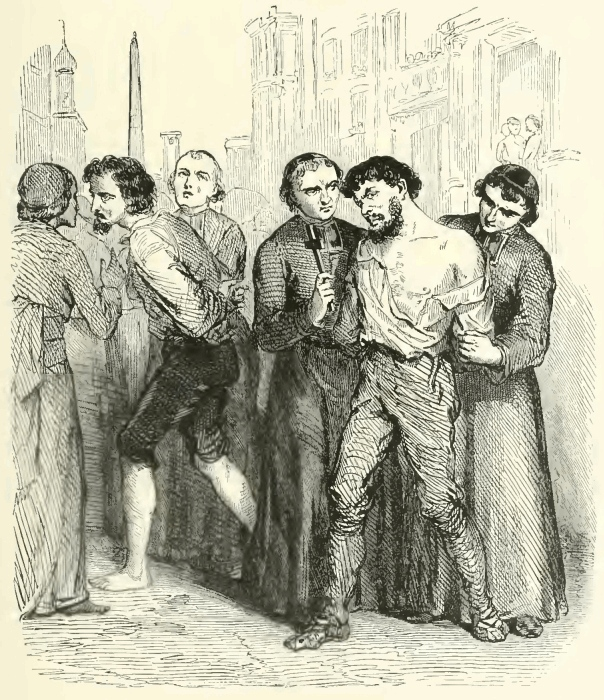
\includegraphics[width=\textwidth]{20167m.jpg}
\end{figure}

“As you left the choice of your costumes to me,” said the count to the
two friends, “I have had these brought, as they will be the most worn
this year; and they are most suitable, on account of the \textit{confetti}
(sweetmeats), as they do not show the flour.”

Franz heard the words of the count but imperfectly, and he perhaps did
not fully appreciate this new attention to their wishes; for he was
wholly absorbed by the spectacle that the Piazza del Popolo presented,
and by the terrible instrument that was in the centre.

It was the first time Franz had ever seen a guillotine,—we say
guillotine, because the Roman \textit{mandaïa} is formed on almost the same
model as the French instrument.\footnote[7]{Dr. Guillotin got the idea of
his famous machine from witnessing an execution in Italy.} The knife, which is shaped like a
crescent, that cuts with the convex side, falls from a less height, and
that is all the difference.

Two men, seated on the movable plank on which the victim is laid, were
eating their breakfasts, while waiting for the criminal. Their repast
consisted apparently of bread and sausages. One of them lifted the
plank, took out a flask of wine, drank some, and then passed it to his
companion. These two men were the executioner’s assistants.

At this sight Franz felt the perspiration start forth upon his brow.

The prisoners, transported the previous evening from the Carceri Nuove
to the little church of Santa Maria del Popolo, had passed the night,
each accompanied by two priests, in a chapel closed by a grating,
before which were two sentinels, who were relieved at intervals. A
double line of carbineers, placed on each side of the door of the
church, reached to the scaffold, and formed a circle around it, leaving
a path about ten feet wide, and around the guillotine a space of nearly
a hundred feet.

All the rest of the square was paved with heads. Many women held their
infants on their shoulders, and thus the children had the best view.
The Monte Pincio seemed a vast amphitheatre filled with spectators; the
balconies of the two churches at the corner of the Via del Babuino and
the Via di Ripetta were crammed; the steps even seemed a parti-colored
sea, that was impelled towards the portico; every niche in the wall
held its living statue. What the count said was true—the most curious
spectacle in life is that of death.

And yet, instead of the silence and the solemnity demanded by the
occasion, laughter and jests arose from the crowd. It was evident that
the execution was, in the eyes of the people, only the commencement of
the Carnival.

Suddenly the tumult ceased, as if by magic, and the doors of the church
opened. A brotherhood of penitents, clothed from head to foot in robes
of gray sackcloth, with holes for the eyes, and holding in their hands
lighted tapers, appeared first; the chief marched at the head.

\begin{figure}[ht]
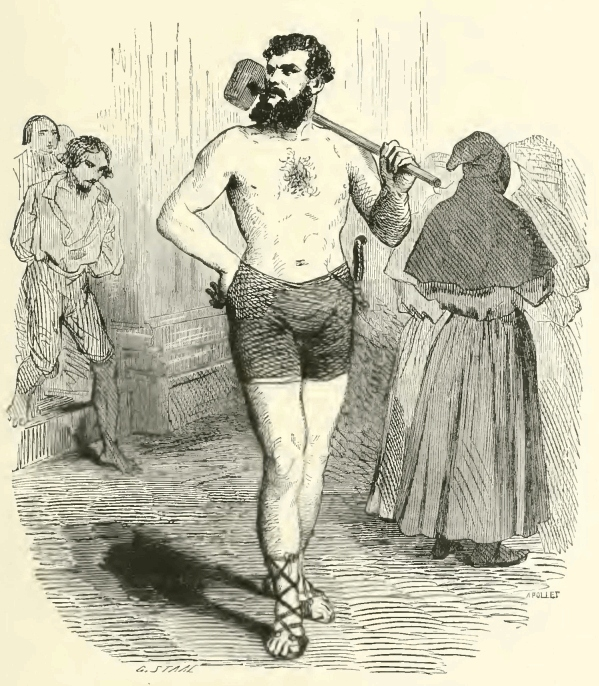
\includegraphics[width=\textwidth]{20169m.jpg}
\end{figure}

Behind the penitents came a man of vast stature and proportions. He was
naked, with the exception of cloth drawers at the left side of which
hung a large knife in a sheath, and he bore on his right shoulder a
heavy iron sledge-hammer.

This man was the executioner.

He had, moreover, sandals bound on his feet by cords.

Behind the executioner came, in the order in which they were to die,
first Peppino and then Andrea. Each was accompanied by two priests.
Neither had his eyes bandaged.

Peppino walked with a firm step, doubtless aware of what awaited him.
Andrea was supported by two priests. Each of them, from time to time,
kissed the crucifix a confessor held out to them.

At this sight alone Franz felt his legs tremble under him. He looked at
Albert—he was as white as his shirt, and mechanically cast away his
cigar, although he had not half smoked it. The count alone seemed
unmoved—nay, more, a slight color seemed striving to rise in his pale
cheeks. His nostrils dilated like those of a wild beast that scents its
prey, and his lips, half opened, disclosed his white teeth, small and
sharp like those of a jackal. And yet his features wore an expression
of smiling tenderness, such as Franz had never before witnessed in
them; his black eyes especially were full of kindness and pity.

However, the two culprits advanced, and as they approached their faces
became visible. Peppino was a handsome young man of four or
five-and-twenty, bronzed by the sun; he carried his head erect, and
seemed on the watch to see on which side his liberator would appear.
Andrea was short and fat; his visage, marked with brutal cruelty, did
not indicate age; he might be thirty. In prison he had suffered his
beard to grow; his head fell on his shoulder, his legs bent beneath
him, and his movements were apparently automatic and unconscious.

“I thought,” said Franz to the count, “that you told me there would be
but one execution.”

“I told you true,” replied he coldly.

“And yet here are two culprits.”

“Yes; but only one of these two is about to die; the other has many
years to live.”

“If the pardon is to come, there is no time to lose.”

“And see, here it is,” said the count. At the moment when Peppino
reached the foot of the \textit{mandaïa}, a priest arrived in some haste,
forced his way through the soldiers, and, advancing to the chief of the
brotherhood, gave him a folded paper. The piercing eye of Peppino had
noticed all. The chief took the paper, unfolded it, and, raising his
hand, “Heaven be praised, and his Holiness also,” said he in a loud
voice; “here is a pardon for one of the prisoners!”

“A pardon!” cried the people with one voice; “a pardon!”

At this cry Andrea raised his head.

“Pardon for whom?” cried he.

Peppino remained breathless.

“A pardon for Peppino, called Rocca Priori,” said the principal friar.
And he passed the paper to the officer commanding the carbineers, who
read and returned it to him.

“For Peppino!” cried Andrea, who seemed roused from the torpor in which
he had been plunged. “Why for him and not for me? We ought to die
together. I was promised he should die with me. You have no right to
put me to death alone. I will not die alone—I will not!”

And he broke from the priests struggling and raving like a wild beast,
and striving desperately to break the cords that bound his hands. The
executioner made a sign, and his two assistants leaped from the
scaffold and seized him.

“What is going on?” asked Franz of the count; for, as all the talk was
in the Roman dialect, he had not perfectly understood it.

“Do you not see?” returned the count, “that this human creature who is
about to die is furious that his fellow-sufferer does not perish with
him? and, were he able, he would rather tear him to pieces with his
teeth and nails than let him enjoy the life he himself is about to be
deprived of. Oh, man, man—race of crocodiles,” cried the count,
extending his clenched hands towards the crowd, “how well do I
recognize you there, and that at all times you are worthy of
yourselves!”

Meanwhile Andrea and the two executioners were struggling on the
ground, and he kept exclaiming, “He ought to die!—he shall die!—I will
not die alone!”

“Look, look,” cried the count, seizing the young men’s hands; “look,
for on my soul it is curious. Here is a man who had resigned himself to
his fate, who was going to the scaffold to die—like a coward, it is
true, but he was about to die without resistance. Do you know what gave
him strength? do you know what consoled him? It was, that another
partook of his punishment—that another partook of his anguish—that
another was to die before him! Lead two sheep to the butcher’s, two
oxen to the slaughterhouse, and make one of them understand that his
companion will not die; the sheep will bleat for pleasure, the ox will
bellow with joy. But man—man, whom God created in his own image—man,
upon whom God has laid his first, his sole commandment, to love his
neighbor—man, to whom God has given a voice to express his
thoughts—what is his first cry when he hears his fellow-man is saved? A
blasphemy. Honor to man, this masterpiece of nature, this king of the
creation!”

And the count burst into a laugh; a terrible laugh, that showed he must
have suffered horribly to be able thus to laugh.

However, the struggle still continued, and it was dreadful to witness.
The two assistants carried Andrea up to the scaffold; the people all
took part against Andrea, and twenty thousand voices cried, “Put him to
death! put him to death!”

Franz sprang back, but the count seized his arm, and held him before
the window.

“What are you doing?” said he. “Do you pity him? If you heard the cry
of ‘Mad dog!’ you would take your gun—you would unhesitatingly shoot
the poor beast, who, after all, was only guilty of having been bitten
by another dog. And yet you pity a man who, without being bitten by one
of his race, has yet murdered his benefactor; and who, now unable to
kill anyone, because his hands are bound, wishes to see his companion
in captivity perish. No, no—look, look!”

\begin{figure}[h]
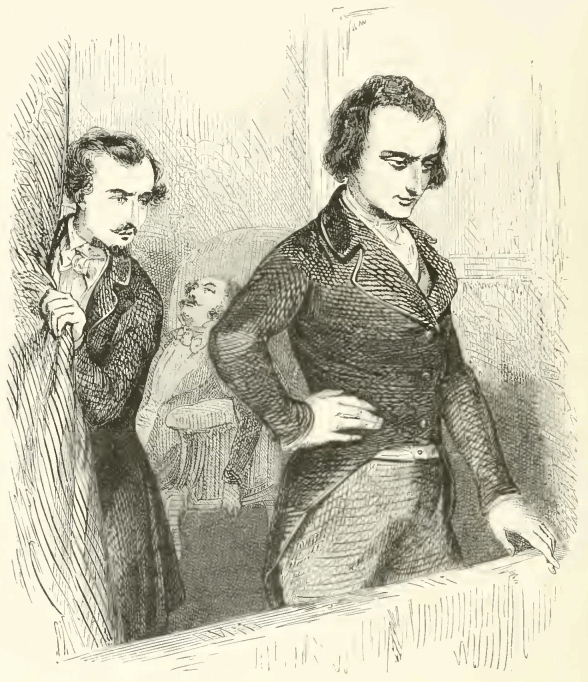
\includegraphics[width=\textwidth]{20172m.jpg}
\end{figure}

The recommendation was needless. Franz was fascinated by the horrible
spectacle.

The two assistants had borne Andrea to the scaffold, and there, in
spite of his struggles, his bites, and his cries, had forced him to his
knees. During this time the executioner had raised his mace, and signed
to them to get out of the way; the criminal strove to rise, but, ere he
had time, the mace fell on his left temple. A dull and heavy sound was
heard, and the man dropped like an ox on his face, and then turned over
on his back.

The executioner let fall his mace, drew his knife, and with one stroke
opened his throat, and mounting on his stomach, stamped violently on it
with his feet. At every stroke a jet of blood sprang from the wound.

This time Franz could contain himself no longer, but sank, half
fainting, into a seat.

Albert, with his eyes closed, was standing grasping the
window-curtains.

The count was erect and triumphant, like the Avenging Angel!
